\section{Ransac mit Maskierung \dcfirstauthorshort} 
\label{sec:maskenbau}
\label{sec:polynombasierte_fahrspurerkennung:ransac}

Aus einem Foto mittels \gls{acr:ransac} eine mathematische Approximation einer Fahrbahnmarkierung zu erhalten, war die von uns anfangs angestrebte Herangehensweise. Der nun folgend beschriebene Ansatz zur Detektion der Fahrbahnlinien ist jedoch in der endgültigen Implementierung nicht zum Einsatz gekommen. Da wir uns jedoch geraume Zeit damit beschäftigt und viele später weiter verwendete Grundfunktionen aufgebaut haben, sollen die Vorgehensweise und die zum Ausschluss der Methode geführten Probleme näher erläutert werden. 

\subsection{Approximation der Straßenmarkierungen}

Ausgangspunkt für die Ermittlung einer passenden Funktion ist das binarisierte Bild, welches nach den in Abbildung~\ref{fig:bildvorverarbeitung_ueberblick} dargestellten Schritten der Bildvorverarbeitung vorliegt. Alle Pixel mit dem Wert \glqq 1\grqq{} stellen im Idealfall potenzielle Linienpunkte dar. Diese sind der richtigen Kategorie \glqq linke\grqq , \glqq mittlere\grqq{} oder \glqq rechte\grqq{} Linie zuzuordnen, wenn sie nicht bereits mittels \gls{acr:ransac}-Algorithmus als Outlier (siehe Abschnitt \ref{ssec:grunglagen:ransac:ablauf}) markiert wurden. Dazu wird je nach Zugehörigkeit eine entsprechende \gls{acr:roi} im Bild festgelegt. Anschließend wird der in Kapitel~\ref{ssec:grunglagen:ransac:ablauf} beschriebene \gls{acr:ransac}-Algorithmus in dem durch die \gls{acr:roi} bestimmten Bildausschnitt durchgeführt.

% Bilder der drei Masken über binarisiertem Bild incl. Fit für linke, mittlere und rechte Linie
\begin{figure}[htbp]
	\centering
	\subfloat[][]{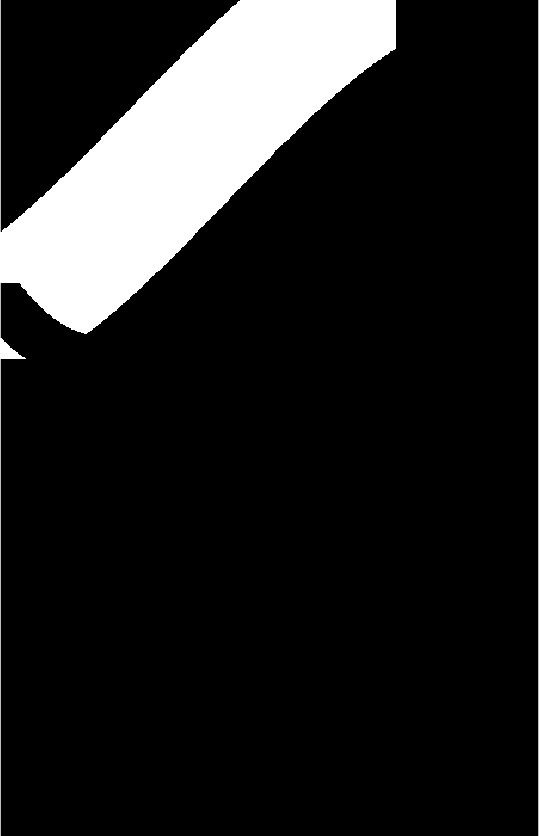
\includegraphics[width=0.32\textwidth]{fahrspurerkennung_ransac_imgMaskLeft.png}}
	\hfill
	\subfloat[][]{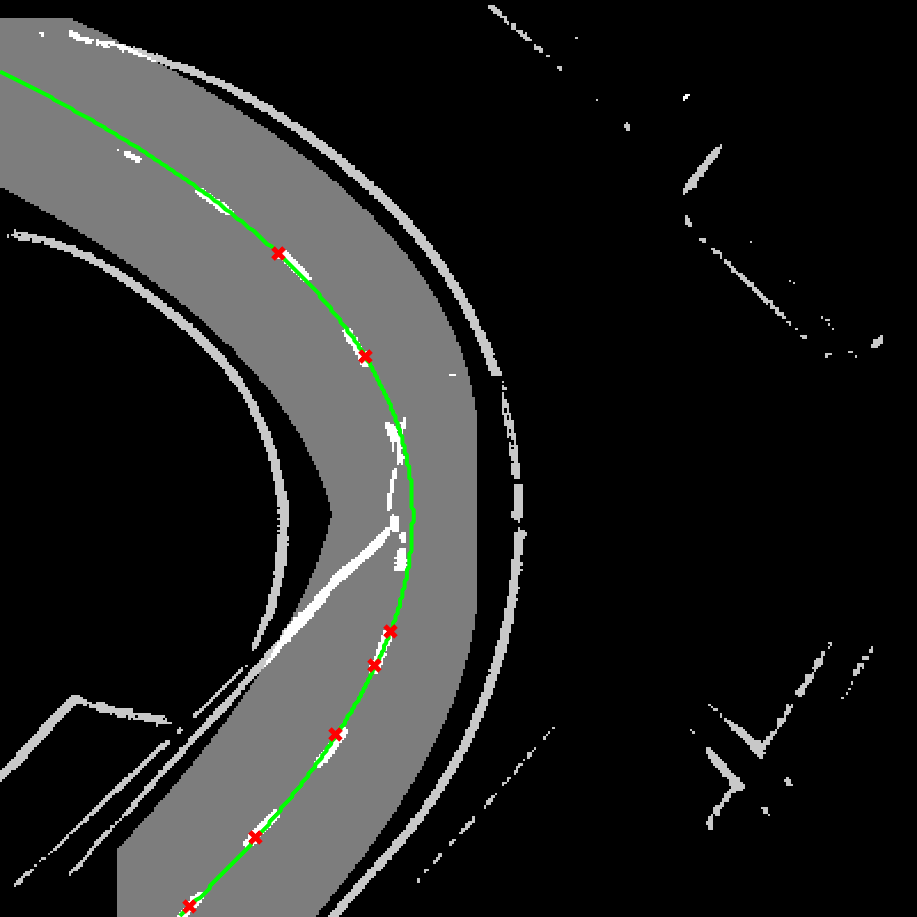
\includegraphics[width=0.32\textwidth]{fahrspurerkennung_ransac_imgMaskMiddle.png}}
	\hfill
	\subfloat[][]{
\includegraphics[width=0.32\textwidth]{fahrspurerkennung_ransac_imgMaskRight.png}}
	\caption{Approximation der linken (a), mittleren (b) und rechten (c) Fahrbahnmarkierung durch ein Polynom dritten Grades mithilfe jeweiliger \glspl{acr:roi} und der Anwendung von \gls{acr:ransac}}
	\label{fig:fahrspurerkennung_ransac_masken}
\end{figure} 

Wie in Abbildung~\ref{fig:fahrspurerkennung_ransac_masken} zu sehen, folgt die Approximaxtion dem Verlauf der Fahrbahnlinien relativ gut. Die eingezeichnete grüne Funktion beschreibt das Ergebnis des Fit eines Polynoms dritten Grades durch die von \gls{acr:ransac} bestimmten Inlier. Mit einem gewissen Abstand verteilt werden anschließend auf dem Polynom potentielle Kartenpunkte diskretisiert, welche einzig dann in die Karte aufgenommen werden, wenn sie sowohl Teil der Funktion sind als auch mit weißen Pixeln des maskierten Bildes übereinstimmen. So wird verhindert, Punkte an stark abweichenden Stellen der Approximation zur echten Fahrbahnmarkierung in die Weltkarte einzutragen. 


\subsection{Bestimmung der \glqq Regions of Interest\grqq{}}

Um die zu einer Linie zugehörigen Pixel an der erwarteten Stelle suchen zu können, wird für jede der drei Fahrbahnmarkierungen eine passende Maske erstellt, welche den Bildausschnitt für \gls{acr:ransac} markiert. Diese \glspl{acr:roi} werden mittels der bereits eingetragenen Kartenpunkte und der Pose zum Zeitpunkt der Bildaufnahme gebildet.  
%Die Weltkarte ist ein Struktur-Feld, in dem unter anderem die Koordinaten der eingetragenen Linienpunkte gespeichert sind, jedoch nicht deren approximierte Funktion. 
Dazu werden eine bestimmte Anzahl der zuletzt eingetragenen Kartenpunkte gleichartiger Kategorie in das aktuelle Bild transformiert, welche folgend die Grundlage für eine Regression darstellen. Die daraus ermittelte Funktion bildet die Mitte der \gls{acr:roi}. Nach einer Dilatation des im Bildausschnitt liegenden Teils der Funktion um einen Parameterwert entsteht ein dickes Band aus Punkten, welche die \gls{acr:roi} beschreiben (siehe Abbildung~\ref{fig:fahrspurerkennung_ransac_masken}).

\subsection{Initialer Maskenbau} 
\label{par:maskenbau:initial}

Ein nicht zu vernachlässigendes Problem stellt allerdings die Initialisierung dar. Wie gewinnt man die Masken, wenn bisher keine Linienpunkte in die Karte eingetragen worden sind? Die einfachste und am Anfang auch implementierte Möglichkeit bietet die aus Parameterwerten vorgeschriebene Maske einer Gerade, in der Annahme, das Auto starte immer auf einem geraden Abschnitt. Da so aber die Robustheit der Linienerkennung schlecht gewährleistet wäre, wurde dies schnell verworfen und eine bessere Möglichkeit gefunden. 

\paragraph{\gls{acr:roi} für die Mittellinie}

% Textumflossenes Bild des ''Ringfilter''-Kerns
\begin{wrapfigure}{r}{0.5\textwidth}
	\centering
	
\includegraphics[width=0.3\textwidth]{fahrspurerkennung_ransac_midfilter.png}
	\caption{Der Kern des \\ \glqq Ringfilters\grqq}
	\label{fig:fahrspurerkennung_ransac_midfilter}
\end{wrapfigure} 

Die gestrichelte Mittellinie besitzt im gesamten, binarisierten Bild Alleinstellungsmerkmale, die sich durch ein darauf angepasstes, weiteres Faltungsfilter nutzen lassen. Die Idee für den in Abbildung~\ref{fig:fahrspurerkennung_ransac_midfilter} gezeigten Filterkern wurde aus \autocite{drauschkeEchtzeitfaehigeStartpunktalgorithmenFuer2016} entnommen. Der im folgenden als \glqq Ringfilter\grqq{} bezeichnete Kern wurde aus einem Innen- und Außenkreis entworfen, sodass der Radius des inneren Kreises mindestens so groß wie die Länge eines Mittellinienstriches im Bild und der Außenkreisradius maximal so groß wie der kürzeste Abstand zwischen zwei Mittellinienstrichen ist. Was als Filterergebnis beispielhaft entsteht, ist in (c) der Abbildung~\ref{fig:fahrspurerkennung_ransac_binarisieren} zu erkennen. Das Filter bewirkt, dass im Ergebnisbild genau dann ein Pixel mit \glqq 1\grqq{} beschrieben wird, wenn der Filterring um dieses Pixel mindestens einen Punkt im binarisierten Bild schneidet. Es entstehen abgegrenzte Bereiche mit einer \glqq 0\grqq{} als Filterantwort genau dann, wenn Mittellinienstriche innerhalb des \glqq Ringfilters\grqq{} liegen und kein weiteres Pixel auf dem Ring um diese Striche gefunden wird. 

% entzerrtes und binarisiertes Beispielbild und Filterergebnisse für Mittellinie nebeneinander (4 Bilder)
\begin{figure}[htbp]
	\centering
	\subfloat[][]{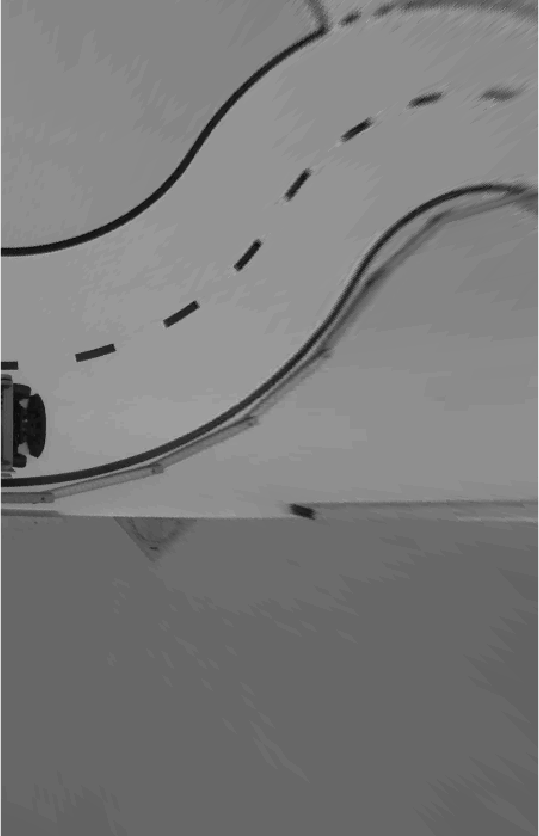
\includegraphics[width=0.47\textwidth]{fahrspurerkennung_ransac_imgUndist.png}}
	\hfill
	\subfloat[][]{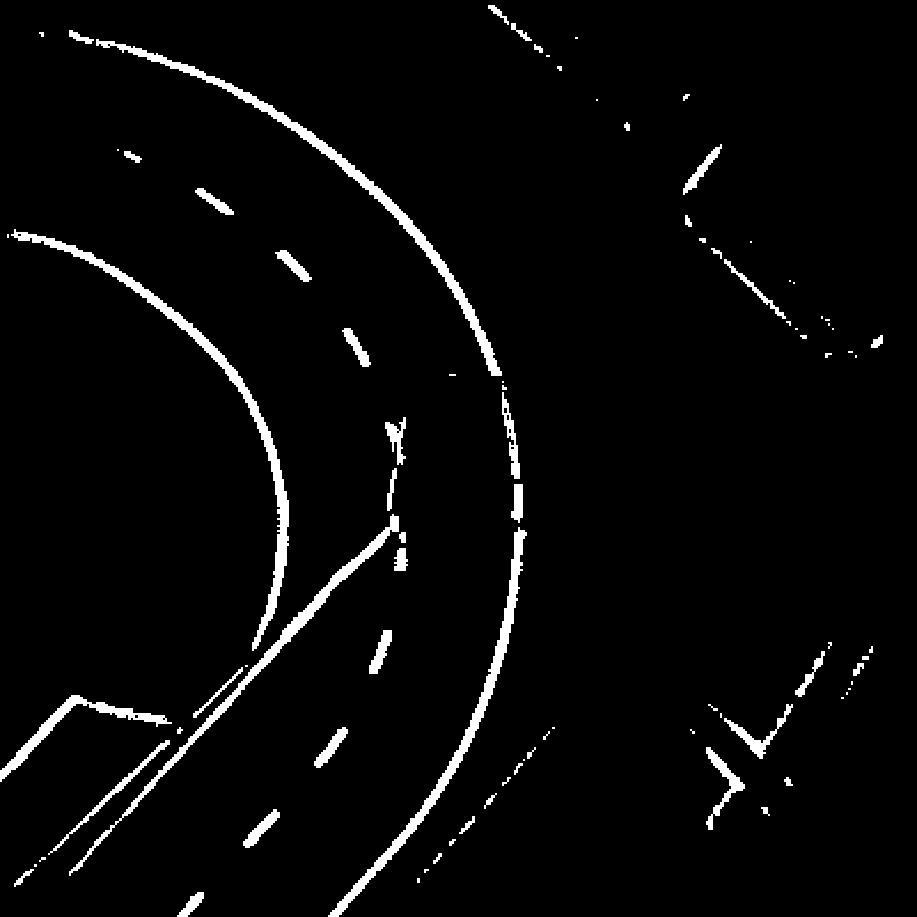
\includegraphics[width=0.47\textwidth]{fahrspurerkennung_ransac_imgBinarized.png}}
	\hfill
	\subfloat[][]{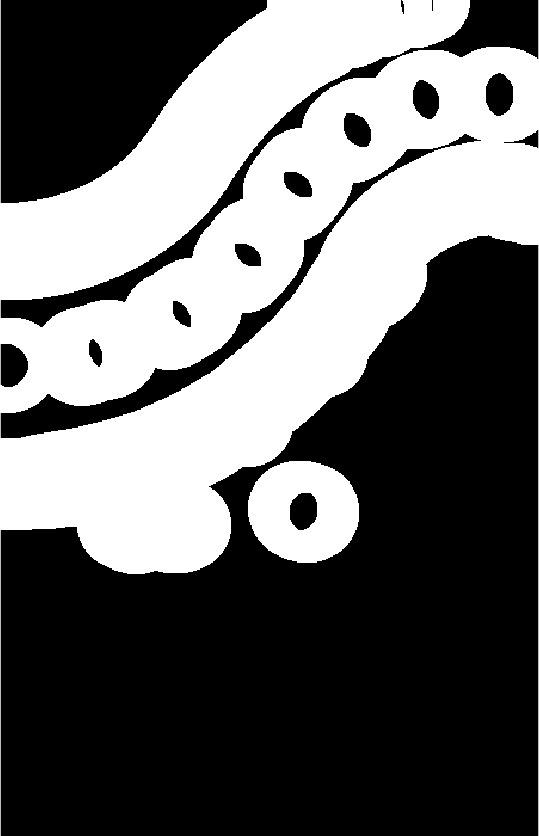
\includegraphics[width=0.47\textwidth]{fahrspurerkennung_ransac_imgMidFiltered.png}}
	\hfill
	\subfloat[][]{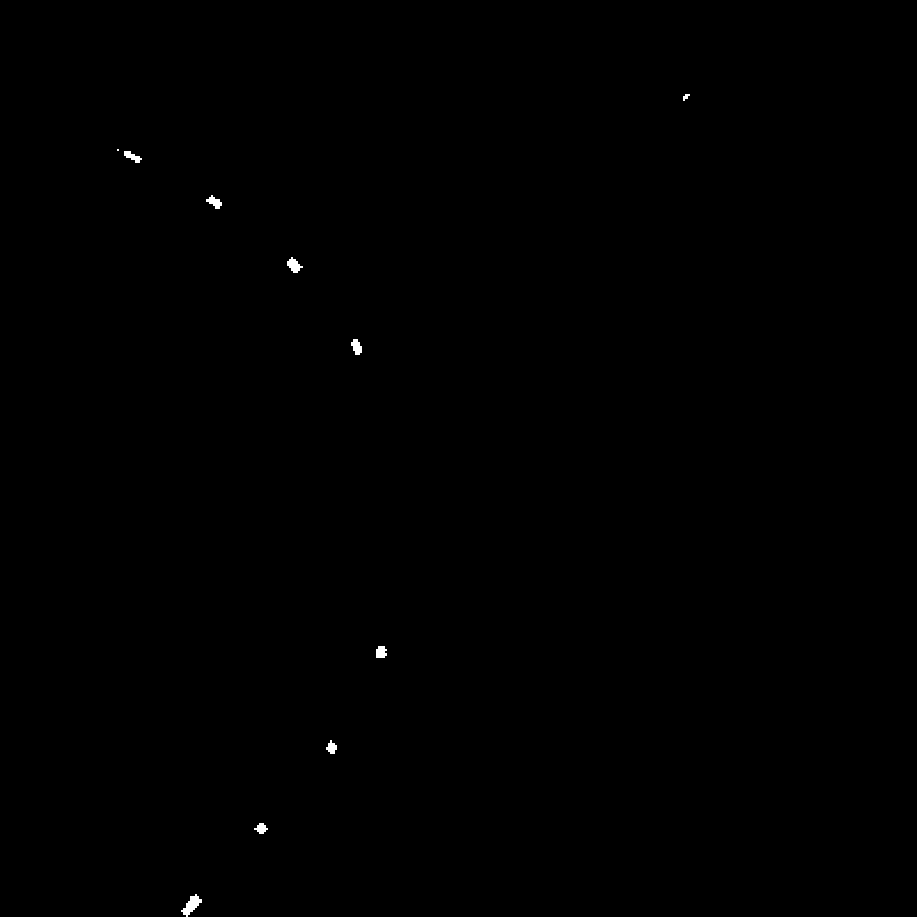
\includegraphics[width=0.47\textwidth]{fahrspurerkennung_ransac_imgBinarizedAndNotImgMidFiltered.png}}
	\caption{entzerrtes (a) und binarisiertes Bild (b) einer Testaufnahme auf der Strecke in alten Kameraeinstellungen; Filterergebnis des ''Ringfilters'' (c) und Durchschnitt dessen Negation mit dem binarisierten Bild (d)}
	\label{fig:fahrspurerkennung_ransac_binarisieren}
\end{figure} 

Die Negation des Filterergebnisses als Maske auf das binarisierte Bild gelegt erzeugt eine Grafik, die allein Pixel aus Punktgruppen enthält, die dem \glqq Ringfilter\grqq{} entsprechend festgelegte Maximallängen und Mindestabstände zu anderen Punkten besitzen. Darauf kann nun der \gls{acr:ransac}-Algorithmus angewendet werden. 
%Dass hier der Einsatz von \gls{acr:ransac} sinnvoll und notwendig ist, erkennt man in (d) der Abbildung~\ref{fig:fahrspurerkennung_ransac_binarisieren} im unteren Teil des Bildes an der hellen Pixelgruppe, welche nicht zur mittleren Fahrbahnmarkierung gehört.

\paragraph{Randlinienmasken}

Die zwei initialen \glspl{acr:roi} für die Randlinien werden anschließend aus der approximierten Funktion dritten Grades der Mittellinie gebildet. Dies geschieht aus der gerichteten Verschiebung diskreter Punkte der Approximation. Gleichung~\eqref{eq:polynom3} sei eine mathematische Beschreibung der Funktion, die den Linienverlauf approximiert, dann ist Gleichung~\eqref{eq:derr_polynom3} die Ableitung, welche den Anstieg an den Stellen \gls{x} beschreibt. Der Verschiebungsvektor \gls{lat:dv} steht dann senkrecht auf \( \mathrm{f} \).

\begin{subequations}
\begin{eqnarray}
\mathrm{f}(\gls{x}) & = & a{\gls{x}}^3 + b{\gls{x}}^2 +c{\gls{x}} +d  \label{eq:polynom3} 	\\
%\mathrm{f}’(\gls{x}) & = & 3a{\gls{x}}^2 + 2b\gls{x} +c \label{eq:derr_polynom3} 							\\
\der{\fnfop}(\gls{x}) & = & 3a{\gls{x}}^2 + 2b\gls{x} +c \label{eq:derr_polynom3} 							\\
\gls{lat:dv} & = & \frac{1}{\sqrt{(-\der{\fnfop}(\gls{x}))^2 + 1}} \cdot
\begin{pmatrix}
-\der{\fnfop}(\gls{x}) 	\\
1 		\\
\end{pmatrix}
\label{eq:maske_verschiebungsvektor}									\\
\begin{pmatrix}
{\gls{x}}_s 	\\
{\gls{y}}_s	\\
\end{pmatrix}
 & = & 
 \begin{pmatrix}
\gls{x} 	\\
\gls{y}	\\
\end{pmatrix}
\pm b_F \cdot \gls{lat:dv}  
\label{eq:maske_randpunkte}
\end{eqnarray}
\end{subequations}

Die Normierung von \gls{lat:dv} multipliziert mit der bekannten Fahrspurbreite \( b_F \) addiert auf den Mittellinienpunkt \( (\gls{x},\gls{y}) \) ergibt einen Stützpunkt \( ({\gls{x}}_s,{\gls{y}}_s) \) der linken (\( + \)) bzw. der rechten (\( - \)) Randlinie (Gleichungen \eqref{eq:maske_verschiebungsvektor} und \eqref{eq:maske_randpunkte}).

Durch die so verschobenen Stützpunkte der erwarteten Lage der Randlinien werden ein neuer Fit und eine anschließende Dilatation vorgenommen, um die initialen Randmasken zu erzeugen. Um auszuschließen, dass man zur mittleren Strichlinie zugehörige Bildpunkte einer Randlinie zuordnet, wird zusätzlich eine elementweise UND-Operation mit der negierten Mittellinienmaske durchgeführt. Die verhinderte Überschneidung der Masken ist auch in Abbildung~\ref{fig:fahrspurerkennung_ransac_masken} zu erkennen.

%––––––––––––––––––––––––––––––––––––––––––––––––––––––
% \section{Ransac mit Maskierung \dcfirstauthorshort}

\subsection{Vorteile von Ransac mit Maskierung}

Eine kubische Funktion als mathematisches Modell der gesuchten Linie bietet einige Vorteile:
\begin{itemize}
\item Im Gegensatz zu einer Geraden, einem Kreis oder einer quadratischen Funktion kann das gewählte Polynom dritten Grades zusätzlich dem Verlauf einer S-Kurve (Übergang einer Links- in eine Rechtskurve und umgekehrt) relativ gut folgen. 
%\item Unter der Annahme einer guten Annäherung zur echten Markierung kann im Falle eines unbrauchbaren Fotos durch Extrapolation trotzdem weitergefahren werden. 
\item Unter der Annahme einer guten Annäherung zur echten Markierung kann durch Extrapolation eine wahrscheinliche Vorhersage des Linienverlaufs in einem später aufgenommenen Bild getroffen werden. 
\item Die Stetigkeit der kubischen Funktion verhindert das plötzliche Abknicken des Linienverlaufs, sodass nahezu senkrecht auftreffende Querstraßenmarkierungen nicht als Kurve erkannt werden
\item Durch die Anwendung von \gls{acr:ransac} haben Unterbrechungen oder kleine Störungen keinen negativen Einfluss. Als Outlier erkannte Pixel werden in der anschließenden Regression nicht berücksichtigt (s. Kapitel~\ref{ssec:grunglagen:ransac:ablauf}).
\end{itemize}

\subsection{Probleme}
\label{ssec:evaluation:ransac:probleme}
Trotz der vielen Vorzüge bringt gerade \gls{acr:ransac} das Problem mit sich, dass drei zu bestimmende, unabhängige Polynome in einem Bildausschnitt zu rechenintensiv und damit zeitaufwendig wären. Daher müssen in einer Aufnahme drei sinnvoll gewählte Bereiche feststehen, in welchen je ein \gls{acr:ransac}-Algorithmus ausgeführt werden kann. 
Das größte Problem, welches letztlich zum Ausschluss der \gls{acr:ransac}-Methode geführt hat, ist die zuverlässige Bestimmung dieser \gls{acr:roi}. Ab Steigung von mehr als 45\(^\circ\) approximiert das Polynom den Linienverlauf deutlich schlechter. 

Entgegen der Erwartungen sind die Extrapolationseigenschaften von Polynomen zum Maskenbau ungeeignet. Da deren Wertebereich stets gegen unendlich läuft, weicht die Funktion am Bildrand meist stärker von der zu erkennenden Kurve ab. Dies führt zu falsch vorhergesagten \glspl{acr:roi}, welche beispielhaft in Abb.~\ref{fig:evaluation_ransac_ransac} dargestellt sind.

\begin{figure}[htbp]
	\centering
	\subfloat[][]{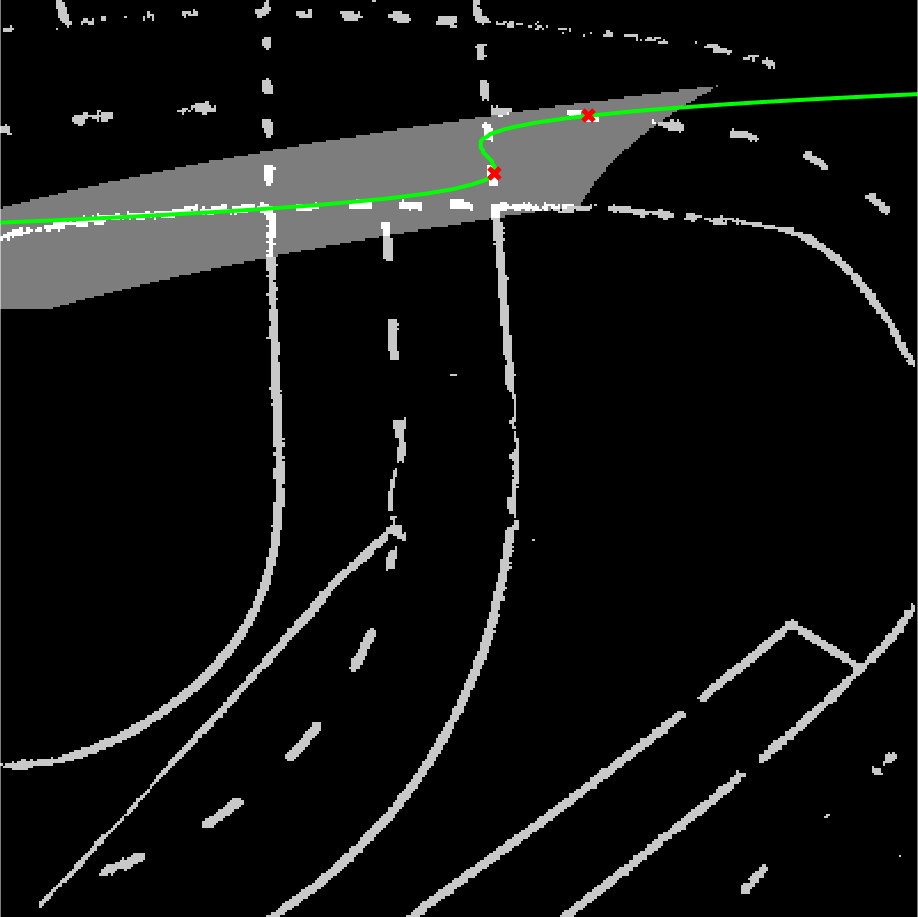
\includegraphics[width=0.32\textwidth]{evaluation_ransac_imgMaskLeft.png}}
	\hfill
	\subfloat[][]{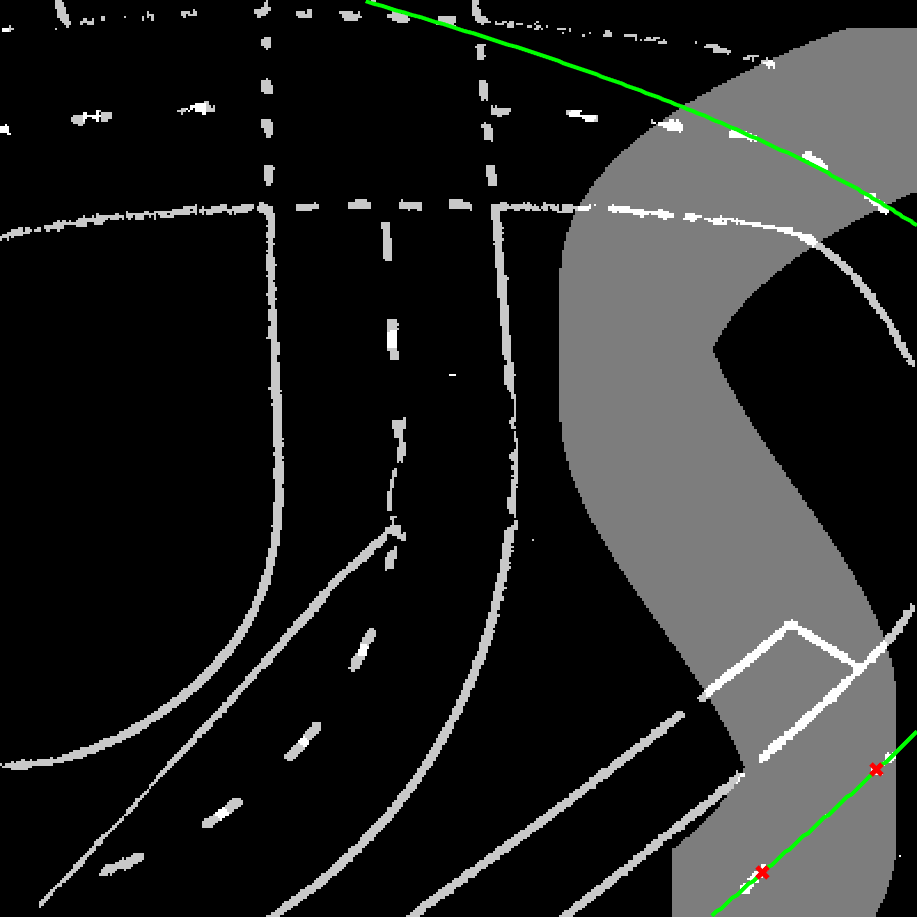
\includegraphics[width=0.32\textwidth]{evaluation_ransac_imgMaskMiddle.png}}
	\hfill
	\subfloat[][]{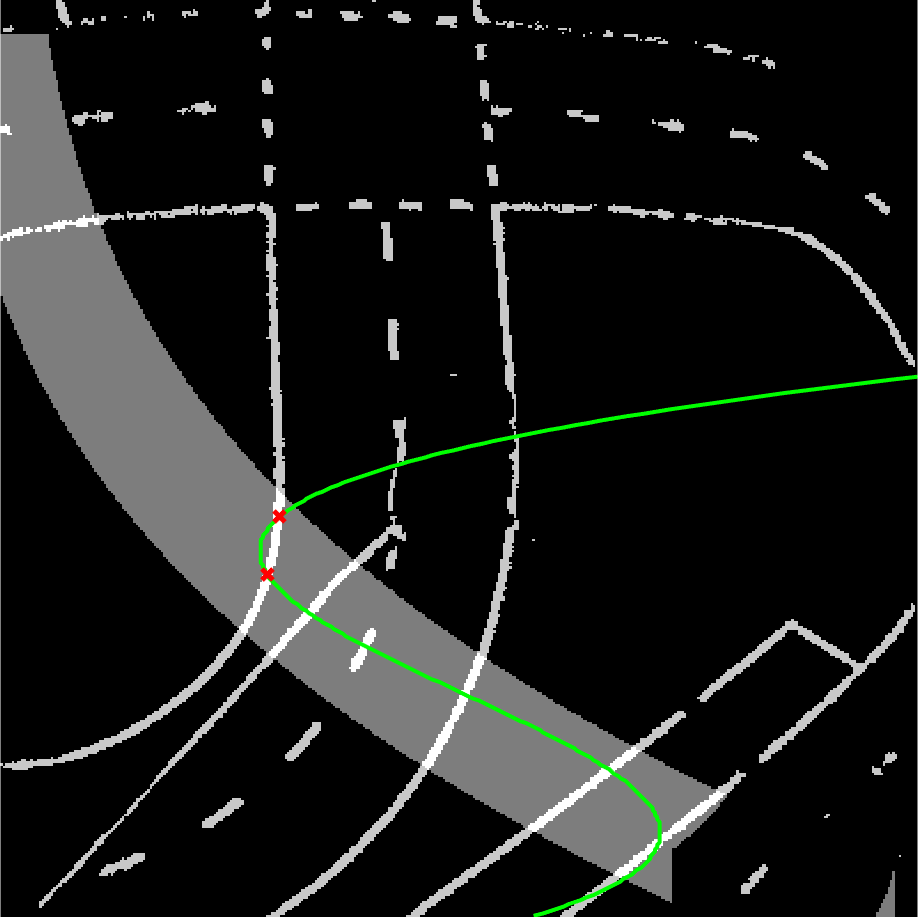
\includegraphics[width=0.32\textwidth]{evaluation_ransac_imgMaskRight.png}}
	\caption{Fehlerhaft erzeugte Masken der linken (a), mittleren (b) und rechten (c) Fahrbahnmarkierungen während eines Testlaufes. In Abb.~\ref{evaluation_ransac_weltkarte} ist der Ausschnitt des Geschehens markiert}
	\label{fig:evaluation_ransac_ransac}
\end{figure} 

Das Polynom hat keine Chance, die Fahrbahnmarkierung richtig abzubilden, da sie nicht zu den Punkten des maskierten Bereichs gehört. Jene fehlerhaften \glspl{acr:roi} entstehen durch zuvor falsch erkannte, in die Weltkarte eingetragene Punkte. Abbildung~\ref{evaluation_ransac_weltkarte} zeigt das Ergebnis eines Testlaufs. Dieser wurde mit Hilfe einer Aufnahme (rosbag\footnote{Rosbag ist eine Reihe von Tools zum Aufnehmen und Wiedergeben von ROS-Topics (wiki.ros.org/rosbag)}) durchgeführt, welche während manueller Steuerung des Fahrzeugs entstanden ist. Im dargestellten Plot der Weltkarte ist die anfänglich zufriedenstellende Detektion der Fahrbahnmarkierungen zu erkennen, welche jedoch ab der ersten Kreuzung verloren geht.

% Bild/Plot der eingetragenen Punkte in der Weltkarte nach ein paar Sekunden
\begin{figure}[htbp] % [htb]
	\centering
	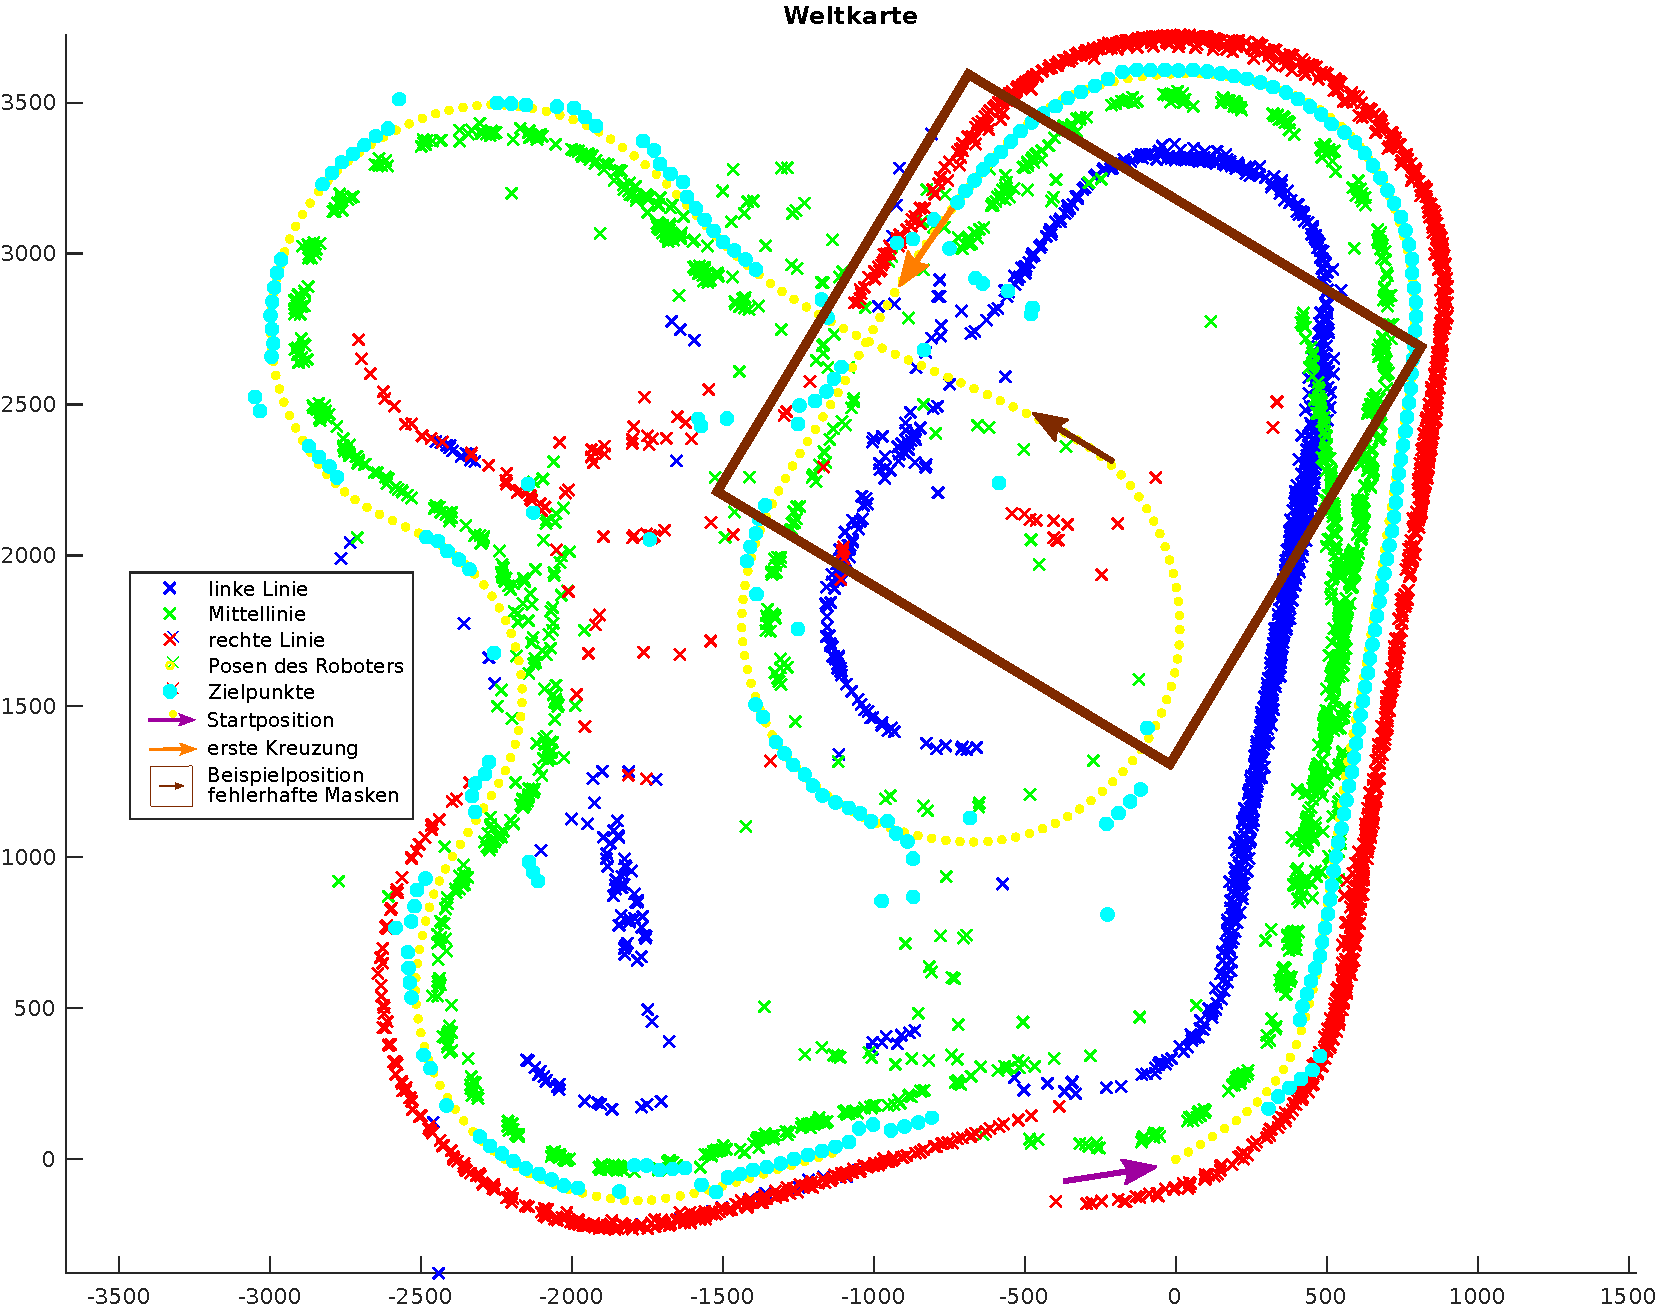
\includegraphics[width=1\textwidth]{evaluation_ransac_worldMap.pdf}
	\caption{Plot der Weltkarte nach einer Testrunde mittels manueller Steuerung}
	\label{evaluation_ransac_weltkarte}
\end{figure} 

Wenn in einem zuletzt untersuchten Bild keine Linienpunkte gefunden wurden, muss die Maske des übernächsten Bildes aus den zuletzt eingetragenen Punkten erstellt werden. Diese Punkte können ungünstigerweise weit von der jetzigen Position entfernt liegen, sodass stark extrapoliert werden muss. In dieser Entfernung zu den Stützstellen bildet das die Maske beschreibende Polynom den wirklichen Linienverlauf ungenügend ab und der \gls{acr:ransac} kann erneut keine richtigen Punkte finden. Somit ist die Voraussetzung gegeben, dass der Algorithmus im nächsten Foto erneut fehlschlägt, da falsche Punkte in der Karte zu noch stärkeren Abweichungen der Masken gegenüber der eigentlichen Markierung führen. Es entwickelt sich eine Kettenreaktion, die ein \glqq Sich-Wieder-Fangen\grqq{} des Algorithmus sehr unwahrscheinlich macht. 
Hinzu kommt, dass selbst bei ideal ausgewählten \glspl{acr:roi} die mathematische Beschreibung nicht jedem beliebigen Kurvenverlauf exakt folgen kann. 


\subsection{Fazit und Lösungsmöglichkeiten}

Durch unser Paradigma, eine Weltkarte aufzubauen, ist der Gedanke naheliegend, deren Information zur Verarbeitung eines Bildes zu nutzen. Voraussetzung dafür ist allerdings, dass die Informationen der Karte hinreichend genau sind. Zugegebenerweise könnte der \gls{acr:ransac} mit Maskierungen zu einem stabilen Verfahren ausgebaut werden, wenn eine Möglichkeit gefunden wird, die Bestimmung der \gls{acr:roi} zuverlässiger zu gestalten. Die Riverflow-Methode bot allerdings die vielversprechende Aussicht auf eine robustere Funktionsweise ohne aufwändige Anpassungen. 

Beispielsweise wäre es denkbar, die maximale Krümmung des kubischen Polynoms zu beschränken, um so ein Abdriften der Masken an Kreuzungen zu unterbinden. Da ein Polynom jedoch stets ins Unendliche läuft, wäre eine andere mathematische Beschreibung möglicherweise sinnvoller gewesen. Wenigstens die Masken könnten aus zusammengesetzten Kreisen oder Splines hervorgehen. Außerdem könnte man die Maskenbreite von der Entfernung bekannter Stützstellen abhängig machen, sodass in unbekannten Bereichen auf größerer Fläche gesucht werden kann. Zusätzlich wäre es möglich, die Masken durch die bekannte Fahrspurbreite voneinander abhängig zu machen, um ein Überlappen oder Vertauschen von linker und rechter Linie zu verhindern.

Falls im Rahmen weiterer Projekte der Riverflow-Algorithmus an seine Grenzen kommen sollte, ließe sich also unser erster Ansatz ebenfalls zum lauffähigen Programm erweitern. Unsere weitere Idee zur Verbesserung der Prädiktion einer Linie wird im nun folgenden Abschnitt zum Kalman beschrieben.

